\documentclass[11pt,a4paper]{article}
\usepackage[T1]{fontenc}
\usepackage[utf8]{inputenc}
\usepackage{mathptmx}
\usepackage[margin=2.5cm]{geometry}
\usepackage{amsmath,amssymb}
\usepackage{graphicx}
\usepackage{booktabs,tabularx,multirow}
\usepackage{threeparttable}
\usepackage{tikz}
\usetikzlibrary{positioning,arrows.meta,shapes.geometric,fit,patterns,decorations.pathreplacing}
\usepackage[authoryear,round]{natbib}
\usepackage{setspace}
\usepackage{xcolor}
\usepackage[colorlinks=true,linkcolor=blue!50!black,citecolor=blue!50!black,urlcolor=blue!50!black]{hyperref}
\onehalfspacing
\newcolumntype{Y}{>{\raggedright\arraybackslash}X}

\title{\textbf{Measuring the Operational Resilience of FinTech Ecosystems in Sub-Saharan Africa: The AFRO-FINRES Framework and Evidence from Cameroon and the CEMAC Region}}
\author{Achaire Zogo Abouma Zozime\textsuperscript{1,*} and Edit Kamel Djupsa\textsuperscript{2}\\[2pt]
\small \textsuperscript{1}University of Yaound\'e I, Yaound\'e, Cameroon\quad \textsuperscript{2}Independent Researcher, Cameroon\\
\small \textsuperscript{*}Correspondence: \href{mailto:achaire.zogo@facsciences-uy1.cm}{achaire.zogo@facsciences-uy1.cm}}
\date{}

\begin{document}
\maketitle

\begin{abstract}
\noindent
Digital financial services have become critical infrastructure in Sub-Saharan Africa, yet no comparative instrument measures whether national FinTech ecosystems can prevent, absorb and recover from operational disruptions. This study develops AFRO-FINRES (African FinTech Operational Resilience Framework), a design-science framework that integrates cybersecurity, recovery and continuity, financial governance and third-party infrastructure redundancy into six dimensions: prevention, detection, response, recovery and continuity, governance, and third-party/shared-infrastructure redundancy. The dimensions are operationalised with 15 indicators drawn exclusively from public sources (ITU Global Cybersecurity Index 2024, World Bank WDI and Worldwide Governance Indicators, Enterprise Surveys and PeeringDB) and aggregated into a 0--100 composite index for 48 Sub-Saharan African countries. Index scores range from 3.6 to 96.5 (mean 43.6). The CEMAC region averages 30.2, and Cameroon scores 45.2 (rank 25/48), with detection capability as its binding constraint. The index is internally consistent (Cronbach's $\alpha=0.86$) and robust to alternative weighting and aggregation (rank correlations 0.97--0.99; 5000 Monte Carlo draws). It is associated with account ownership ($\rho=0.75$) and mobile-money ownership ($\rho=0.45$) from the Global Findex 2025, and these associations persist after controlling for income. An illustrative stress-test module translates dimension gaps into recovery trajectories. The framework provides supervisors with a transparent, replicable diagnostic tool and a basis for prioritising resilience investments.
\end{abstract}

\noindent\textbf{Keywords:} operational resilience; cybersecurity; FinTech; mobile money; composite indicator; financial governance; third-party risk; Sub-Saharan Africa; CEMAC; Cameroon

\noindent\textbf{JEL codes:} G21, G28, O33, O55, L86

\section{Introduction}

Mobile money and other FinTech services have changed how households and firms in Sub-Saharan Africa (SSA) save, pay and transfer value. Evidence from Kenya shows that mobile money lowers transaction costs, improves risk sharing and reduces poverty \citep{Jack2014,Suri2016}. Across the continent, mobile-money adoption has been a main driver of financial inclusion \citep{Ahmad2020,Lashitew2019}. In Cameroon, the Global Findex 2025 database (2024 survey wave) reports that 60.9\% of adults hold an account and 55.1\% hold a mobile-money account \citep{WB2025Findex}. Payment platforms, agent networks, application programming interfaces (APIs), telecommunications networks, cloud services and data centres now form an interdependent system. When one of these components fails, the effects reach millions of users who often have no alternative to cash.

This dependence makes \emph{operational resilience}, the ability of an organisation or system to deliver critical services through disruption, a financial-stability concern. International standard setters have formalised the concept. Examples include the Basel Committee's \emph{Principles for Operational Resilience} \citep{BCBS2021}, the CPMI--IOSCO cyber-resilience guidance for financial market infrastructures \citep{CPMI2016}, the Financial Stability Board's third-party risk toolkit \citep{FSB2023} and the European Union's Digital Operational Resilience Act \citep[DORA;][]{EU2022DORA}. Cyber risk is now considered a potential source of systemic risk \citep{Kopp2017,Bouveret2018,Aldasoro2022}. Most of this work, however, is designed for advanced economies with mature supervisory data. It focuses on individual institutions rather than national ecosystems, and it seldom considers African conditions such as unreliable power supply, limited Internet exchange infrastructure, a small cybersecurity workforce and uneven institutional quality \citep{Kshetri2019}.

The academic literature has three gaps. First, studies of FinTech in Africa mostly examine adoption, inclusion and welfare \citep{Ozili2018,Ahmad2020,Johnen2023}. Fewer address the continuity and security of the services being adopted. Second, studies of cyber and operational resilience in finance are mostly conceptual or institution-level \citep{Dupont2019,Milkau2021,Iyer2024}, or quantify losses with proprietary data \citep{Bouveret2019}. They do not provide a cross-country measure that regulators in data-scarce environments can calculate. Third, existing composite indices cover their own domains, such as cybersecurity commitment \citep{ITU2024GCI} and governance \citep{Kaufmann2011}, but none combines prevention, detection, response, continuity, governance and third-party dependencies into one measure of resilience capacity for digital finance. The Central African Economic and Monetary Community (CEMAC) is especially understudied, even though it shares a single central bank and regional payment infrastructure. Recent survey evidence from Cameroon shows that perceived cybersecurity and trust shape continued use of mobile money \citep{Mvogo2026}, but ecosystem-level evidence is still lacking.

This paper addresses these gaps with three research questions:
\begin{description}
  \item[RQ1] How can the operational resilience of national FinTech ecosystems be conceptualised and measured using only publicly available data?
  \item[RQ2] How do SSA countries, the CEMAC region and Cameroon perform, and which dimensions constrain their resilience?
  \item[RQ3] Is the resulting measure statistically robust, and is it associated with digital-finance outcomes as theory predicts?
\end{description}

We follow a design-science approach \citep{Hevner2004,Peffers2007} and build a conceptual framework from multidisciplinary literature \citep{Jabareen2009}. The resulting artefact, AFRO-FINRES, links resilience engineering \citep{Holling1973,Bruneau2003,Linkov2018}, cybersecurity management \citep{NIST2024}, continuity planning \citep{Swanson2010,ISO22301}, and financial governance and third-party risk regulation \citep{BCBS2021,FSB2023}. We operationalise it as a composite index following the OECD--JRC methodology \citep{OECD2008}. We compute the index for 48 SSA countries, test its robustness with uncertainty and sensitivity analysis \citep{Saisana2005,Greco2018}, check its association with Global Findex outcomes, and add a scenario-based stress-test module.

The paper makes three contributions. Conceptually, it proposes an integrated six-dimension model that treats cybersecurity, continuity, governance and third-party dependencies as complementary parts of one resilience capability. Methodologically, it provides a transparent and fully reproducible index built from open data, which regulators and researchers in data-scarce settings can update each year. Empirically, it provides the first comparative resilience mapping of SSA digital-finance ecosystems, with a detailed diagnosis of Cameroon and the CEMAC region. The paper does not claim to measure realised fraud or outages. The index measures \emph{resilience-enabling capacity}, and we discuss the limits of this interpretation explicitly.

The remainder of the paper is organised as follows. Section~\ref{sec:background} reviews the literature and develops the framework. Section~\ref{sec:methods} describes the data and index construction. Section~\ref{sec:results} presents the results. Section~\ref{sec:discussion} discusses implications and limitations, and Section~\ref{sec:conclusion} concludes.

\section{Literature Review and Conceptual Framework}\label{sec:background}

\subsection{From Resilience Theory to Operational Resilience in Finance}

In ecology, resilience originally meant the capacity of a system to absorb change and still persist \citep{Holling1973}. Engineering research made the concept measurable. \citet{Bruneau2003} represent the resilience of critical infrastructure as the loss of service functionality over time after a shock, which depends on robustness, redundancy, resourcefulness and rapidity. \citet{Linkov2018} apply this logic to cyber systems and define cyber resilience as the ability to plan for, absorb, recover from and adapt to adverse cyber events. In operations management, \citet{Annarelli2016} describe operational resilience as a strategic capability that combines static (preventive) and dynamic (reactive) elements.

In financial regulation, operational resilience extends operational risk management. Operational risk management aims to reduce the probability and impact of losses. Operational resilience assumes that disruptions will happen and focuses on keeping critical services within tolerance levels \citep{BCBS2021,Milkau2021}. Qualitative research shows that practitioners consider resilience a cross-functional capability that requires governance, mapping of critical services and third-party oversight \citep{Iyer2024}. \citet{Dupont2019} argues that the cyber-resilience of financial institutions depends on the wider ecosystem of suppliers, regulators and law enforcement, so ecosystem-level analysis is needed.

\subsection{Cyber Risk, FinTech and Systemic Vulnerability}

Cyber incidents can damage financial stability through loss of confidence, lack of substitutes for critical services and interconnectedness \citep{Kopp2017}. Quantitative assessments suggest that cyber losses for financial institutions are economically significant and have fat tails \citep{Bouveret2018,Bouveret2019}. Cyber risk is related to firm size, digitalisation and the sector of activity \citep{Aldasoro2022}. FinTech increases these exposures because new entrants, platforms and API-based business models create new technological dependencies \citep{Gomber2018,Chen2022,Vucinic2022}. Concentration on a few cloud and technology providers creates single points of failure \citep{Gulliver2023,FSB2023}. These concerns led to the EU's DORA regime \citep{EU2022DORA}.

In Africa, \citet{Kshetri2019} documents a fast-changing cybercrime landscape alongside weak institutional and technical capacity. The ITU Global Cybersecurity Index (GCI) shows large differences in national cybersecurity commitment across the continent \citep{ITU2024GCI}. These differences reflect country-group characteristics such as income and institutional development \citep{Donalds2022}. Consumer-protection frameworks for digital financial services are still uneven \citep{DiCastri2023}.

\subsection{Trust, Infrastructure and Digital-Finance Adoption}

Adoption research shows that trust and perceived security drive continued use of mobile payments \citep{Cao2018}. In Cameroon, \citet{Mvogo2026} find that cybersecurity and trust affect customers' continued use of mobile money. Infrastructure is also important. Mobile-money adoption depends on network coverage, electricity and complementary infrastructure \citep{Mothobi2017}, on the diffusion of mobile phones and on institutional quality \citep{Lashitew2019}. Interoperability affects how far mobile money spreads \citep{Brunnermeier2023}, and agent networks determine accessibility \citep{Johnen2023}. If resilience-enabling capacities support trust and service availability, they should be associated with higher use of digital finance. This idea is the basis for our external validation.

\subsection{The AFRO-FINRES Framework}

Using concept-mapping procedures \citep{Jabareen2009}, we combined the resilience cycle (anticipate, absorb, recover, adapt), the five functions of the NIST Cybersecurity Framework 2.0 plus its new \emph{Govern} function \citep{NIST2024}, continuity-planning standards \citep{Swanson2010,ISO22301,ISO27001} and prudential principles on operational resilience and third-party risk \citep{BCBS2021,FSB2023,CPMI2016}. The resulting framework has six dimensions (Figure~\ref{fig:framework}).

\begin{figure}[htbp]
\centering
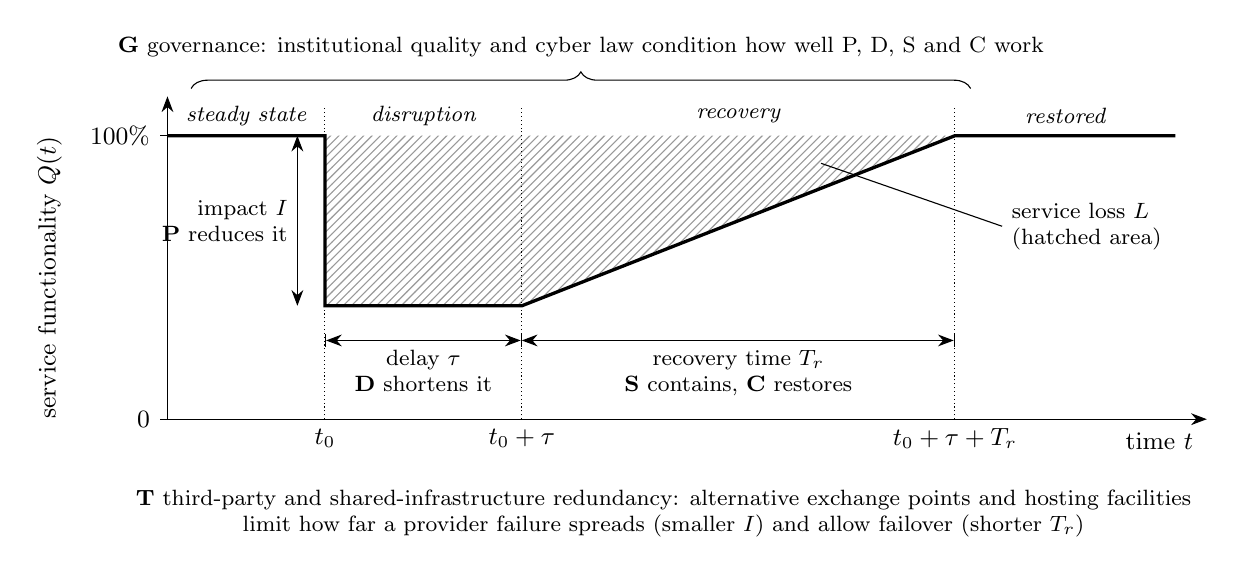
\begin{tikzpicture}[font=\small,>={Stealth[length=2mm]}]
\draw[->] (0,0) -- (13.2,0) node[below left=2pt]{time $t$};
\draw[->] (0,0) -- (0,4.1);
\node[rotate=90] at (-1.5,1.8) {service functionality $Q(t)$};
\draw (0.1,3.6) -- (-0.1,3.6) node[left]{100\%};
\draw (0.1,0) -- (-0.1,0) node[left]{0};
\fill[pattern=north east lines,pattern color=black!40] (2,3.6) -- (2,1.44) -- (4.5,1.44) -- (10,3.6) -- cycle;
\draw[very thick] (0,3.6) -- (2,3.6) -- (2,1.44) -- (4.5,1.44) -- (10,3.6) -- (12.8,3.6);
\foreach \x in {2,4.5,10} \draw[densely dotted] (\x,0) -- (\x,3.95);
\node[below] at (2,0) {$t_0$};
\node[below] at (4.5,0) {$t_0+\tau$};
\node[below] at (10,0) {$t_0+\tau+T_r$};
\node[font=\footnotesize\itshape] at (1,3.85) {steady state};
\node[font=\footnotesize\itshape] at (3.25,3.85) {disruption};
\node[font=\footnotesize\itshape] at (7.25,3.85) {recovery};
\node[font=\footnotesize\itshape] at (11.4,3.85) {restored};
\draw[<->] (1.65,3.6) -- (1.65,1.44) node[midway,left,align=right,font=\footnotesize]{impact $I$\\\textbf{P} reduces it};
\draw[|<->|] (2,1.0) -- (4.5,1.0) node[midway,below,align=center,font=\footnotesize]{delay $\tau$\\\textbf{D} shortens it};
\draw[<->|] (4.5,1.0) -- (10,1.0) node[midway,below,align=center,font=\footnotesize]{recovery time $T_r$\\\textbf{S} contains, \textbf{C} restores};
\draw (8.3,3.25) -- (10.6,2.45) node[right,align=left,font=\footnotesize]{service loss $L$\\(hatched area)};
\draw[decorate,decoration={brace,amplitude=6pt}] (0.3,4.2) -- (10.2,4.2) node[midway,above=8pt,align=center,font=\footnotesize]{\textbf{G}~governance: institutional quality and cyber law condition how well P, D, S and C work};
\node[align=center,font=\footnotesize] at (6.3,-1.2) {\textbf{T}~third-party and shared-infrastructure redundancy: alternative exchange points and hosting facilities\\limit how far a provider failure spreads (smaller $I$) and allow failover (shorter $T_r$)};
\end{tikzpicture}
\caption{The AFRO-FINRES conceptual framework, drawn on the service-functionality curve used in the stress-test module (Section~\ref{sec:scen}). Prevention (P) reduces the initial impact $I$, detection (D) shortens the containment delay $\tau$, and response (S) and recovery and continuity (C) shorten the recovery time $T_r$. Governance (G) conditions the effectiveness of these four capabilities. Third-party redundancy (T) limits the propagation of provider failures and allows failover. The hatched area is the service loss $L$.}
\label{fig:framework}
\end{figure}

\textbf{Prevention (P)} covers the capacity to reduce the likelihood and impact of incidents through secure infrastructure, standards and human capital. \textbf{Detection (D)} covers the timely identification of anomalies and attacks, including national computer incident response teams (CIRTs) and technical monitoring. \textbf{Response (S)} covers organisational arrangements for containing incidents and coordinating stakeholders nationally and internationally. \textbf{Recovery and continuity (C)} covers the physical and digital conditions for restoring service, such as reliable power and connectivity. \textbf{Governance (G)} covers the institutional quality and legal framework that shape the incentives, enforcement and accountability of all actors. \textbf{Third-party and shared-infrastructure redundancy (T)} covers the availability of alternative interconnection and hosting options, which limits concentration on single providers.

From this framework we derive six theoretical propositions that guide the design of the index. They are not all directly testable with public data.
\begin{description}
 \item[P1] Higher prevention capacity reduces the initial impact of disruptive events.
 \item[P2] Higher detection capacity shortens the time between incident onset and containment.
 \item[P3] Stronger response and continuity capacities shorten the recovery time.
 \item[P4] Governance quality moderates P1--P3 by strengthening the effectiveness of technical capabilities.
 \item[P5] Greater third-party and shared-infrastructure redundancy reduces the propagation of provider-level failures.
 \item[P6] Ecosystems with higher overall resilience capacity show higher digital-finance use and user trust.
\end{description}
P1--P5 inform the stress-test module (Section~\ref{sec:scen}). P6 is examined empirically through external validation (Section~\ref{sec:valid}).

\section{Materials and Methods}\label{sec:methods}

\subsection{Research Design and Sample}

The study follows the design-science research methodology of \citet{Peffers2007}: problem identification, definition of objectives, design of the artefact, demonstration, evaluation and communication. The artefact is the AFRO-FINRES index. It is demonstrated on the 48 economies classified by the World Bank as Sub-Saharan Africa, including the six CEMAC members (Cameroon, Central African Republic, Chad, Republic of Congo, Equatorial Guinea and Gabon). We evaluate it statistically (internal consistency, uncertainty and sensitivity analysis) and through its external associations.

\subsection{Indicators and Data Sources}

We applied four selection criteria, following \citet{OECD2008}: conceptual relevance to a dimension, public availability, coverage of at least 95\% of the sample, and recency (2024--2025 where possible). Table~\ref{tab:ind} lists the 15 retained indicators. The ITU GCI 2024 reports country scores on five pillars, each with a maximum of 20 points \citep{ITU2024GCI}. These scores were transcribed from the country profiles of the report, checked a second time against the profiles for all 48 countries, and assigned to the dimensions they best represent. The technical pillar, which includes CIRT capability, measures detection. The organisational and cooperation pillars measure response. The capacity-development pillar contributes to prevention, and the legal pillar contributes to governance. The governance dimension also includes the four Worldwide Governance Indicators most relevant to financial supervision and contract enforcement \citep{Kaufmann2011,WB2025WGI}. Continuity uses electricity access, the share of firms experiencing electrical outages (World Bank Enterprise Surveys) and Internet use \citep{WBWDI}. The third-party dimension uses the number of active Internet exchange points (IXPs) and colocation facilities per 10 million inhabitants, taken from PeeringDB \citep{PeeringDB2026}. These counts measure the diversity of shared interconnection and hosting infrastructure available to digital-finance providers.

\begin{table}[htbp]
\centering
\caption{AFRO-FINRES dimensions, indicators and sources.}
\label{tab:ind}
\small
\begin{threeparttable}
\begin{tabularx}{\textwidth}{l l Y l l}
\toprule
Dim. & Code & Indicator & Source & Year \\
\midrule
P & P1 & Secure Internet servers per million people (log) & WDI & 2024 \\
  & P2 & GCI capacity-development pillar (0--20) & ITU GCI & 2024 \\
D & D1 & GCI technical-measures pillar (0--20) & ITU GCI & 2024 \\
S & S1 & GCI organisational-measures pillar (0--20) & ITU GCI & 2024 \\
  & S2 & GCI cooperation-measures pillar (0--20) & ITU GCI & 2024 \\
C & C1 & Access to electricity (\% of population) & WDI & 2024 \\
  & C2 & Firms experiencing electrical outages (\%; $-\ln(1+x)$) & WDI/ES & 2020--25\tnote{a} \\
  & C3 & Individuals using the Internet (\% of population) & WDI & 2017--24\tnote{b} \\
G & G1--G4 & Regulatory quality; government effectiveness; rule of law; control of corruption & WGI & 2025 \\
  & G5 & GCI legal-measures pillar (0--20) & ITU GCI & 2024 \\
T & T1 & Active IXPs per 10 million people, $\ln(1+x)$ & PeeringDB & 2026\tnote{c} \\
  & T2 & Active colocation facilities per 10 million people, $\ln(1+x)$ & PeeringDB & 2026\tnote{c} \\
\bottomrule
\end{tabularx}
\begin{tablenotes}\footnotesize
\item Notes: WDI = World Development Indicators; ES = Enterprise Surveys; WGI = Worldwide Governance Indicators; GCI = Global Cybersecurity Index. Latest available observation per country.
\item[a] Median year 2024; missing for Eritrea and Sudan. \item[b] Median year 2024. \item[c] Snapshot retrieved November 2026; populations from WDI (2025).
\end{tablenotes}
\end{threeparttable}
\end{table}

\subsection{Normalisation, Weighting and Aggregation}

Let $x_{ik}$ be the raw value of indicator $k$ for country $i$. Skewed count variables were log-transformed, and variables where lower values are better were inverted. Each indicator was winsorised at the 2.5th and 97.5th percentiles to limit the influence of outliers. It was then rescaled to 0--100 with min--max normalisation:
\begin{equation}
 y_{ik}=100\,\frac{\tilde{x}_{ik}-\min_j \tilde{x}_{jk}}{\max_j \tilde{x}_{jk}-\min_j \tilde{x}_{jk}},
\end{equation}
where $\tilde{x}_{ik}$ is the winsorised value. Dimension scores are the arithmetic means of their indicators, $d_{im}=\frac{1}{|K_m|}\sum_{k\in K_m} y_{ik}$. For the two countries missing C2, the dimension mean was computed over the available indicators. The baseline index gives equal weight to the six dimensions:
\begin{equation}
 \text{AFRO-FINRES}_i=\sum_{m=1}^{6} w_m\, d_{im},\qquad w_m=\tfrac{1}{6}.
\end{equation}
Equal weighting is the most transparent choice when there is no consensus on the relative importance of the dimensions \citep{OECD2008,Greco2018}. We test three alternative specifications. (i) \emph{Geometric aggregation}, $\prod_m d_{im}^{w_m}$ with $d_{im}$ floored at 1, which limits compensation between dimensions. (ii) \emph{Governance-moderated aggregation}, which formalises P4 by scaling the security dimensions with governance quality:
\begin{equation}
 \text{AFRO-FINRES}^{mod}_i=\tfrac{1}{6}\Big[d_{iS}+d_{iC}+d_{iT}+d_{iG}+(d_{iP}+d_{iD})\big(1-\lambda+\lambda\tfrac{d_{iG}}{100}\big)\Big],\quad \lambda=0.5.
\end{equation}
(iii) \emph{PCA weighting}, where weights are proportional to the squared loadings on the first principal component of the dimension correlation matrix.

\subsection{Robustness, Uncertainty and Sensitivity Analysis}

Following \citet{Saisana2005}, we ran 5000 Monte Carlo simulations. Each simulation draws (a) dimension weights from a symmetric Dirichlet distribution ($\alpha=4$, so weights vary around equality), (b) a normalisation method (min--max or z-score) and (c) an aggregation rule (arithmetic or geometric), each with equal probability. For every country we report the median simulated rank and the 5th--95th percentile interval. We also ran a leave-one-dimension-out analysis and computed Cronbach's $\alpha$ across the six dimensions.

\subsection{External Validation}\label{sec:valid_m}

To examine P6, we correlated the index with Global Findex 2025 outcomes \citep{WB2025Findex}: account ownership, mobile-money account ownership, the share of adults who pay cash in stores because they do not trust card or phone payments, phone-lock use and perceived adequacy of mobile money. Only observations from 2021 or later were used. We used Spearman's rank correlation, which is robust for small samples ($n=33$--36). Because both resilience capacity and financial inclusion increase with income, we also computed partial rank correlations controlling for log GDP per capita (PPP).

\subsection{Scenario-Based Stress-Test Module}\label{sec:scen_m}

To make the index useful for supervisors, we translate dimension scores into stylised recovery trajectories with the functionality-loss approach of \citet{Bruneau2003}. Let $Q(t)\in[0,100]$ denote the service functionality of the digital-finance ecosystem. An incident at $t=0$ removes a share $I$ of functionality, which remains degraded until detection and containment at time $\tau$ and then recovers linearly over $T_r$. With normalised dimension scores $\hat d_m=d_m/100$ and a governance multiplier $g=0.5+0.5\hat d_G$ (P4):
\begin{align}
 I &= I_0\,(1-a\,g\,\hat d_P)\,(1-b\,\hat d_T)^{\mathbb{1}[\text{third-party}]}, \label{eq:I}\\
 \tau &= \tau_0\,(1-c\,g\,\hat d_D), \qquad
 T_r = T_{r0}\,\big(1-e\,g\,(\hat d_S+\hat d_C)/2\big), \label{eq:tau}\\
 L &= \int_0^{\infty}\!\big(100-Q(t)\big)\,dt = I\,\tau + \tfrac{1}{2} I\, T_r . \label{eq:L}
\end{align}
We set $a=0.6$, $b=0.5$, $c=0.7$ and $e=0.6$. We define four scenarios that reflect common threats to African digital finance. SC1 is a phishing/SIM-swap account-takeover campaign ($I_0=25\%$, $\tau_0=72$\,h, $T_{r0}=120$\,h). SC2 is a payment-API provider failure (60\%, 6\,h, 48\,h; third-party). SC3 is an outage of a core mobile-money platform (90\%, 2\,h, 36\,h). SC4 is an attack on a shared switch or central infrastructure (70\%, 24\,h, 96\,h; third-party). The parameters are illustrative assumptions, not empirical estimates. The module shows how the framework can be used and is not a forecast.

\subsection{Reproducibility}

All data were retrieved programmatically from the World Bank API (sources 2, 3 and 28) and the PeeringDB API, or transcribed from the ITU GCI 2024 report. The Python scripts that download the data, build the index, run the robustness analysis and produce every table and figure are provided in the replication package (see Data Availability Statement).

\section{Results}\label{sec:results}

\subsection{Resilience Landscape in Sub-Saharan Africa}

Figure~\ref{fig:rank} ranks all 48 countries. Index scores range from 3.6 (Central African Republic) to 96.5 (Mauritius), with a mean of 43.6 and a median of 45.2 (SD 21.0). A leading group scores above 70: Mauritius, South Africa (76.2), Botswana (75.2), Ghana (74.4), Rwanda (74.0), Tanzania (71.1), Kenya (71.1) and Cabo Verde (70.7). These countries combine high GCI scores with strong governance or infrastructure. The weakest performers are fragile or conflict-affected states: the Central African Republic, Eritrea (5.7), Guinea-Bissau (12.0), Burundi (13.7) and South Sudan (17.1). Across the region, response is the strongest dimension (mean 59.1) and third-party redundancy is the weakest (27.4). Detection is the most dispersed dimension (SD 37.2), so incident-detection capacity separates the ecosystems more than any other capability.

\begin{figure}[htbp]
\centering
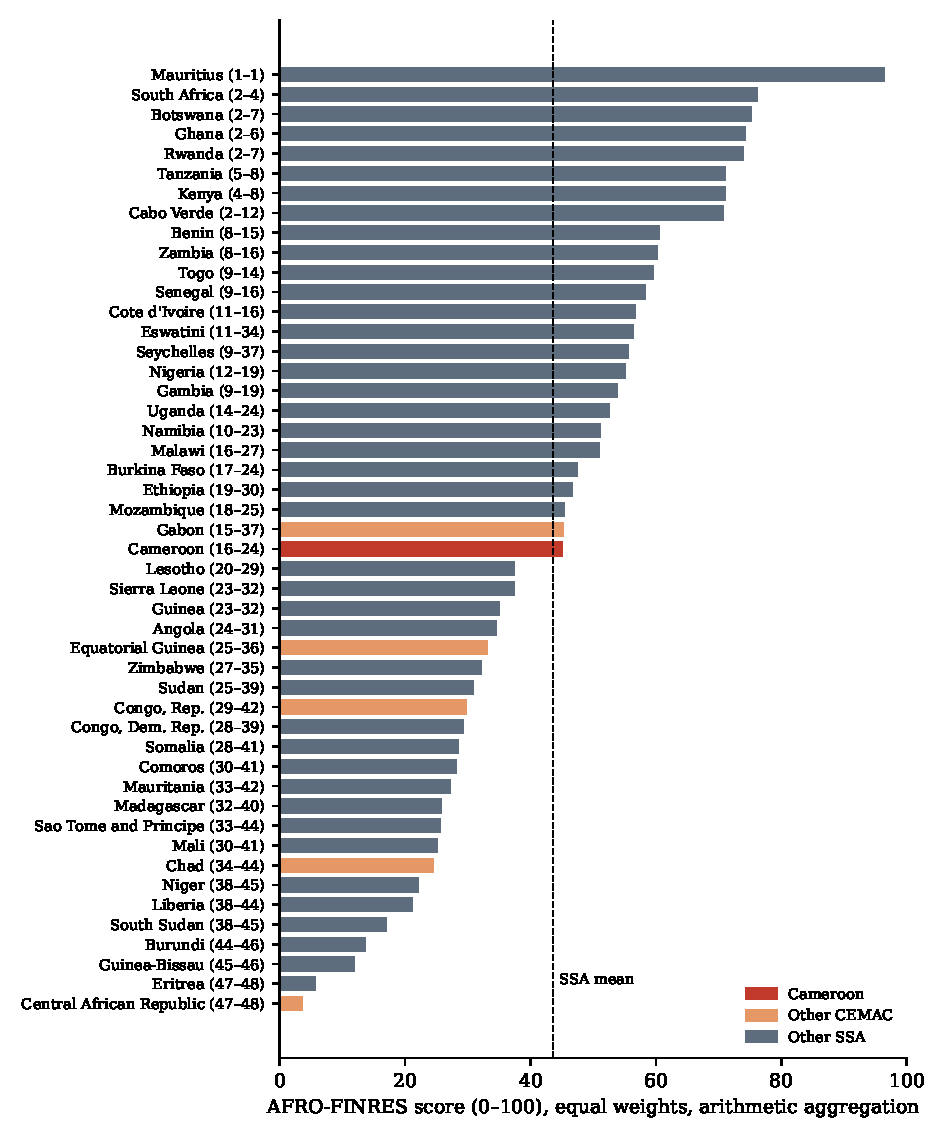
\includegraphics[width=0.92\textwidth]{fig2_ranking.pdf}
\caption{AFRO-FINRES scores for 48 Sub-Saharan African countries (equal weights). Cameroon and other CEMAC members are highlighted; parentheses give the 5th--95th percentile Monte Carlo rank interval.}
\label{fig:rank}
\end{figure}

\subsection{Cameroon and the CEMAC Region}

The CEMAC region averages 30.2, which is 13.4 points below the SSA mean (Table~\ref{tab:cemac}). Its average detection score is especially low (9.0 versus 43.6 for SSA), and it also trails in prevention (22.8 versus 38.1) and governance (33.8 versus 51.3). The region scores above the SSA average only in third-party redundancy (37.8 versus 27.4). This result mainly reflects Gabon (83.2) and the Republic of Congo (61.2), whose small populations increase per-capita infrastructure counts.

Cameroon scores 45.2 and ranks 25th, level with Gabon and ahead of the other CEMAC members. Its profile is uneven (Figure~\ref{fig:radar}). Response is a relative strength (67.5, above the SSA mean), reflecting the organisational and cooperation pillars of the GCI. Detection is the binding constraint (31.0), consistent with a GCI technical-pillar score of only 6.18/20 and the country's Tier~3 (``Establishing'') classification \citep{ITU2024GCI}. Governance (46.1) and continuity (40.9) are slightly below the regional average, reflecting WGI estimates between $-0.79$ and $-1.20$, electricity access of 72\% and Internet use of 46\%. With three active IXPs and seven colocation facilities, Cameroon scores 36.2 on third-party redundancy, above the SSA mean. Gabon matches Cameroon's composite score with a very different profile: it scores zero on detection and very high on redundancy. The two cases illustrate that one composite score can hide different vulnerabilities.

\begin{table}[htbp]
\centering
\caption{AFRO-FINRES dimension scores, composite index and rank uncertainty: CEMAC members and benchmarks.}
\label{tab:cemac}
\small
\begin{threeparttable}
\begin{tabular}{l rrrrrr r r c}
\toprule
Country & P & D & S & C & G & T & Index & Rank & MC rank [5--95\%] \\
\midrule
Cameroon & 49.2 & 31.0 & 67.5 & 40.9 & 46.1 & 36.2 & 45.2 & 25 & 21 [16--24] \\
Gabon & 33.0 & 0.0 & 36.5 & 63.0 & 55.5 & 83.2 & 45.2 & 24 & 25 [15--37] \\
Equatorial Guinea & 24.5 & 7.0 & 37.3 & 79.6 & 19.5 & 30.7 & 33.1 & 30 & 31 [25--36] \\
Congo, Rep. & 12.9 & 0.0 & 31.0 & 40.4 & 33.2 & 61.2 & 29.8 & 33 & 37 [29--42] \\
Chad & 17.4 & 15.9 & 63.6 & 1.9 & 32.9 & 15.4 & 24.5 & 41 & 39 [34--44] \\
Central African Rep. & 0.0 & 0.0 & 0.0 & 5.8 & 15.6 & 0.0 & 3.6 & 48 & 48 [47--48] \\
\midrule
CEMAC mean & 22.8 & 9.0 & 39.3 & 38.6 & 33.8 & 37.8 & 30.2 & -- & -- \\
SSA mean & 38.1 & 43.6 & 59.1 & 41.9 & 51.3 & 27.4 & 43.6 & -- & -- \\
\midrule
Kenya & 79.8 & 95.6 & 100.0 & 44.9 & 65.3 & 40.7 & 71.1 & 7 & 7 [4--8] \\
Ghana & 65.6 & 100.0 & 100.0 & 69.0 & 78.8 & 32.6 & 74.4 & 4 & 5 [2--6] \\
Rwanda & 73.9 & 95.2 & 98.4 & 48.4 & 91.1 & 37.0 & 74.0 & 5 & 5 [3--7] \\
Mauritius & 89.9 & 100.0 & 100.0 & 92.8 & 96.3 & 100.0 & 96.5 & 1 & 1 [1--1] \\
\bottomrule
\end{tabular}
\begin{tablenotes}\footnotesize
\item Notes: P = prevention; D = detection; S = response; C = recovery and continuity; G = governance; T = third-party/shared-infrastructure redundancy. Scores 0--100. MC = median Monte Carlo rank and 5th--95th percentile interval over 5000 simulations.
\end{tablenotes}
\end{threeparttable}
\end{table}

\begin{figure}[htbp]
\centering
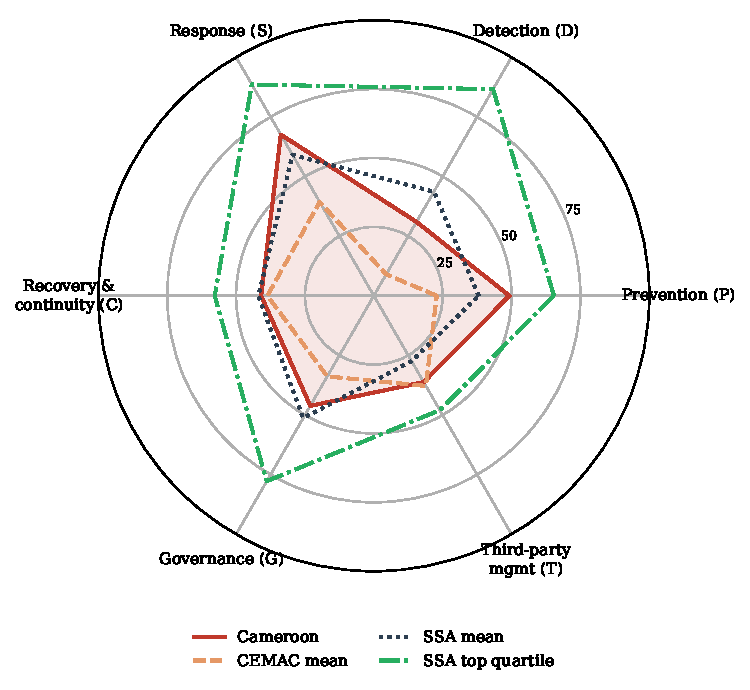
\includegraphics[width=0.62\textwidth]{fig3_radar.pdf}
\caption{Dimension profile of Cameroon compared with the CEMAC mean, the SSA mean and the SSA top quartile.}
\label{fig:radar}
\end{figure}

\subsection{Statistical Coherence and Robustness}

The six dimensions are internally consistent (Cronbach's $\alpha=0.863$). The first principal component explains 63.0\% of the variance, so a single latent construct is a reasonable summary. A second component (19.9\%) separates the infrastructure-based dimensions (C, T) from the cyber-capability dimensions (P, D, S). This pattern is confirmed by the low correlations between continuity and detection ($\rho=0.23$) and between continuity and response ($\rho=0.20$). The PCA-derived weights (P 0.242, G 0.211, S 0.197, D 0.174, C 0.088, T 0.088) give less weight to infrastructure. Even so, the country ranking hardly changes (Table~\ref{tab:robust}). The rank correlation between the baseline and each alternative specification is 0.967 or higher. When any single dimension is removed, ranks change by 1.0--2.5 positions on average, with maximum shifts of 4--11 positions. Detection and continuity have the largest effects. In the Monte Carlo analysis the median width of the 90\% rank interval is 8 positions. Cameroon's interval (16--24) is narrow, while Gabon's is wide (15--37) because its scores across dimensions are very uneven.

\begin{table}[htbp]
\centering
\caption{Robustness of country rankings to alternative specifications.}
\label{tab:robust}
\small
\begin{tabular}{l c c}
\toprule
Specification & Spearman $\rho$ with baseline & Cameroon rank \\
\midrule
Baseline (equal weights, arithmetic) & 1.000 & 25 \\
Geometric aggregation & 0.967 & -- \\
Governance-moderated ($\lambda=0.5$) & 0.995 & -- \\
PCA weights & 0.986 & -- \\
Monte Carlo (5000 draws), median [5--95\%] & -- & 21 [16--24] \\
\midrule
\multicolumn{3}{l}{Leave-one-dimension-out: mean / max absolute rank shift} \\
\quad without P / D / S & \multicolumn{2}{l}{1.00/5 \quad 2.46/11 \quad 1.96/6} \\
\quad without C / G / T & \multicolumn{2}{l}{2.04/10 \quad 1.58/4 \quad 1.79/9} \\
\bottomrule
\end{tabular}
\end{table}

\subsection{External Validation}\label{sec:valid}

Table~\ref{tab:valid} and Figure~\ref{fig:valid} report the association between the index and digital-finance outcomes. As P6 predicts, higher resilience capacity is strongly associated with account ownership ($\rho=0.746$, $p<0.001$) and moderately associated with mobile-money account ownership ($\rho=0.450$, $p=0.006$). Both associations remain after controlling for income (partial $\rho=0.589$ and $0.333$). Contrary to our expectations, the share of adults who pay cash because they distrust card or phone payments is \emph{positively} associated with the index ($\rho=0.456$). The question is only relevant where digital payments are available as an alternative to cash. In low-capacity ecosystems, cash is used because there is no alternative, not because people distrust digital payments, so the indicator mainly captures exposure to digital payments. This interpretation is tentative and needs micro-level testing. Phone-lock use and perceived adequacy of mobile money are not significantly related to the index.

\begin{table}[htbp]
\centering
\caption{Association between AFRO-FINRES and Global Findex 2025 outcomes.}
\label{tab:valid}
\small
\begin{threeparttable}
\begin{tabular}{l c c c c c}
\toprule
Outcome (\% adults) & $n$ & Spearman $\rho$ & $p$ & Partial $\rho$ (ln GDP pc) & $p$ \\
\midrule
Account ownership & 36 & 0.746 & $<$0.001 & 0.589 & $<$0.001 \\
Mobile-money account & 36 & 0.450 & 0.006 & 0.333 & 0.050 \\
Cash use: distrust of card/phone payments & 34 & 0.456 & 0.007 & 0.363 & 0.035 \\
Phone has a lock & 34 & 0.217 & 0.217 & 0.008 & 0.966 \\
Mobile money meets financial needs & 33 & 0.280 & 0.114 & 0.231 & 0.196 \\
\bottomrule
\end{tabular}
\begin{tablenotes}\footnotesize
\item Notes: Findex observations from 2021 onward (mostly 2024 survey waves). Partial correlations control for log GDP per capita (PPP, constant 2021 international \$).
\end{tablenotes}
\end{threeparttable}
\end{table}

\begin{figure}[htbp]
\centering
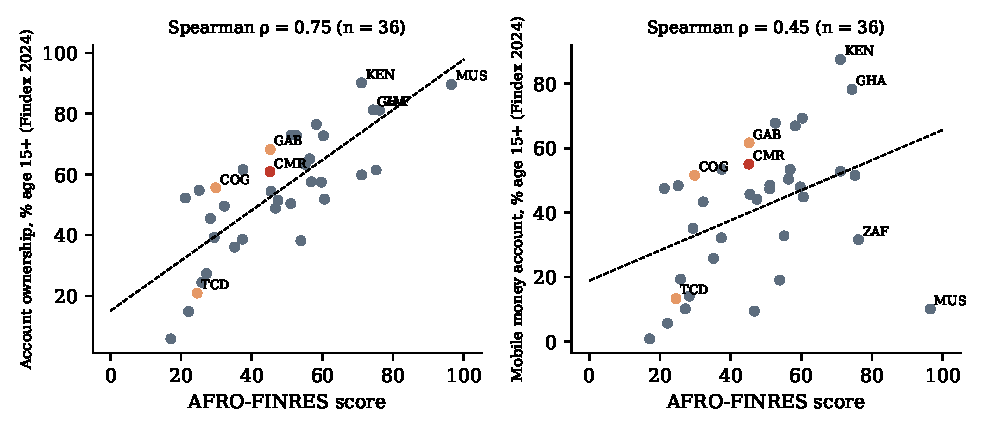
\includegraphics[width=0.95\textwidth]{fig4_validation.pdf}
\caption{AFRO-FINRES versus account ownership and mobile-money account ownership (Global Findex 2025 database, 2024 survey wave). CEMAC members highlighted.}
\label{fig:valid}
\end{figure}

\subsection{Illustrative Stress Tests}\label{sec:scen}

Figure~\ref{fig:scen} and Table~\ref{tab:scen} show the stress-test module for six representative ecosystems. Because the trajectories are computed from dimension scores, they agree closely with the index ranking (Spearman $\rho=-0.996$ between the index and mean simulated loss). This agreement follows from the construction of the module and is not independent validation. The module is useful because it decomposes losses. Under SC1 (account-takeover campaign), Cameroon's functionality loss is 2085 percentage-point-hours, compared with 1066 for Kenya and 570 for Mauritius. Most of the gap comes from the long undetected period ($\tau=60.6$\,h versus 32.2\,h in Kenya). Under SC4 (attack on shared infrastructure), Cameroon's loss (2554) is 21\% higher than Gabon's (2103), because Gabon's greater redundancy limits the initial impact.

\begin{figure}[htbp]
\centering
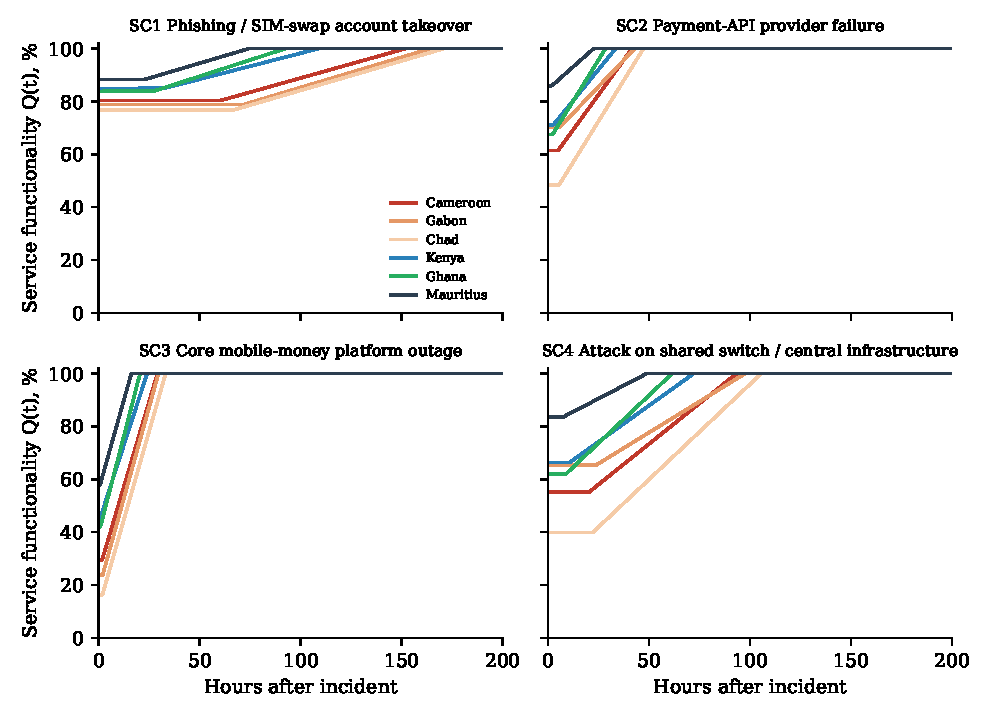
\includegraphics[width=\textwidth]{fig5_scenarios.pdf}
\caption{Illustrative service-functionality trajectories $Q(t)$ under four disruption scenarios. Parameters are stylised assumptions (Section~\ref{sec:scen_m}).}
\label{fig:scen}
\end{figure}

\begin{table}[htbp]
\centering
\caption{Simulated functionality loss $L$ (percentage-point-hours) and the effect of closing Cameroon's dimension gaps.}
\label{tab:scen}
\small
\begin{threeparttable}
\begin{tabular}{l rrrr}
\toprule
 & SC1 & SC2 & SC3 & SC4 \\
\midrule
Mauritius & 570 & 173 & 356 & 465 \\
Ghana & 967 & 500 & 617 & 1337 \\
Kenya & 1066 & 521 & 675 & 1397 \\
Gabon & 2497 & 724 & 1204 & 2103 \\
Cameroon & 2085 & 900 & 1088 & 2554 \\
Chad & 2765 & 1362 & 1466 & 3845 \\
\midrule
\multicolumn{5}{l}{\textit{Cameroon counterfactuals (\% loss reduction):}} \\
\quad D: 31.0 $\rightarrow$ 86.6 (index 54.4) & 19.3 & 7.3 & 3.7 & 12.0 \\
\quad G: 46.1 $\rightarrow$ 77.7 (index 50.4) & 10.9 & 11.7 & 12.0 & 11.4 \\
\quad P: 49.2 $\rightarrow$ 65.4 (index 47.9) & 9.0 & 9.0 & 9.0 & 9.0 \\
\quad S: 67.5 $\rightarrow$ 88.6 (index 48.7) & 2.6 & 4.7 & 5.4 & 3.9 \\
\quad T: 36.2 $\rightarrow$ 47.9 (index 47.1) & 0.0 & 7.2 & 0.0 & 7.2 \\
\quad C: 40.9 $\rightarrow$ 57.7 (index 48.0) & 2.1 & 3.8 & 4.3 & 3.1 \\
\bottomrule
\end{tabular}
\begin{tablenotes}\footnotesize
\item Notes: SC1 phishing/SIM-swap account takeover; SC2 payment-API provider failure; SC3 core mobile-money platform outage; SC4 attack on shared switch/central infrastructure. Counterfactuals raise one dimension to the SSA top-quartile mean. Results depend on the assumed parameters and are illustrative.
\end{tablenotes}
\end{threeparttable}
\end{table}

The counterfactual exercise ranks Cameroon's intervention priorities. Raising detection to the top-quartile level adds the most to the index (+9.2 points) and has the largest effect on fraud-type scenarios (19.3\% lower loss under SC1). Improving governance gives the largest average loss reduction across scenarios (11.5\%), because in the model governance strengthens every technical capability (P4).

\section{Discussion}\label{sec:discussion}

\subsection{Theoretical Implications}

The results support treating operational resilience in digital finance as one multidimensional construct. The dimensions correlate strongly and load on a common factor, but they are not redundant. The second principal component separates \emph{cyber capability} (prevention, detection, response) from \emph{physical and infrastructural continuity} (power, connectivity, interconnection). Supervisory frameworks developed in advanced economies treat infrastructure as given and focus on institutional processes \citep{BCBS2021,EU2022DORA}. In SSA, the infrastructure layer varies independently of cyber capability. Equatorial Guinea, for example, scores well on continuity but poorly on cyber capability, while Chad shows the opposite pattern. An African resilience framework therefore has to model both layers explicitly. This finding extends ecosystem perspectives on cyber resilience \citep{Dupont2019,Linkov2018} to the context of developing economies.

The positive association with account and mobile-money ownership, which remains after controlling for income, is consistent with the view that security and continuity capacities support trust and therefore the use of digital finance \citep{Cao2018,Mvogo2026}. It also complements adoption studies that focus on infrastructure and institutions \citep{Mothobi2017,Lashitew2019}. The cross-sectional design does not allow causal inference. Reverse causality is plausible, because larger digital-finance markets may create incentives to invest in cybersecurity. The unexpected sign of the distrust indicator also shows that survey-based trust measures need careful interpretation when access to digital alternatives differs across countries.

\subsection{Policy Implications for Cameroon and CEMAC}

Four implications follow, subject to the limitations below. First, \emph{detection} is the most urgent gap for Cameroon and the CEMAC region. Strengthening national and sectoral CIRTs, sharing threat intelligence between mobile-network operators, banks and the regulator, and requiring reporting of fraud and incidents would directly address the weakest dimension. Second, \emph{governance} strengthens all other capabilities. Regulatory quality and enforcement determine whether technical controls are used effectively. Third, because CEMAC countries share a central bank and payment infrastructure, a regional resilience framework is a natural step. Such a framework could include mapping of critical services, impact tolerances, third-party registers and scenario testing following \citet{BCBS2021} and \citet{FSB2023}. Fourth, the AFRO-FINRES index can be updated each year from public data, so supervisors could use it as a low-cost monitoring tool and complement it with confidential supervisory data.

\subsection{Limitations and Future Research}

The study has several limitations. (i) \emph{Proxy validity}: the index measures resilience-enabling capacities at national level, not realised resilience of individual FinTech firms or observed fraud and outages. The GCI measures government commitment rather than operational performance. PeeringDB measures the presence of shared infrastructure, not providers' contractual redundancy or concentration on specific vendors. A zero count may also reflect missing registration rather than absence. (ii) \emph{Construct overlap with development}: the index correlates with income ($\rho=0.56$), especially through continuity ($\rho=0.79$). Partial correlations reduce but do not remove this confound. (iii) \emph{Data vintages}: indicators come from 2017--2026, with most observations from 2024--2025. Findex covers only 36 countries. (iv) \emph{Manual transcription}: GCI pillar scores were transcribed from country profiles and checked against the report, but transcription errors cannot be fully excluded. (v) \emph{Scenario parameters} are assumptions. Future work should calibrate them with incident data from regulators, operators or the GSMA. (vi) \emph{Cross-sectional design}: the index cannot yet capture dynamics. Future research could build a panel from earlier GCI editions, validate the index against confidential supervisory incident data, test the propositions at firm level with structural equation modelling using surveys of FinTech managers, and adapt the framework to other monetary unions such as WAEMU.

\section{Conclusions}\label{sec:conclusion}

This paper developed AFRO-FINRES, a framework and composite index that measures the operational-resilience capacity of FinTech ecosystems in Sub-Saharan Africa using only public data. The index integrates prevention, detection, response, continuity, governance and third-party redundancy. It is internally consistent and robust to alternative methods, and it is associated with digital-finance use. Applied to 48 countries, it shows large differences in resilience capacity across the region. The CEMAC region lags by about 13 points, and Cameroon's resilience is limited mainly by weak detection capability and moderate governance quality. The framework makes the resilience of digital finance measurable, comparable and open to policy action. Its transparent and replicable design allows researchers and supervisors to update, critique and extend it as better data become available.

\vspace{1em}
\noindent\textbf{Author Contributions:} Conceptualization, A.Z.A.Z.; methodology, A.Z.A.Z.; writing---original draft preparation, A.Z.A.Z. and E.K.D.; writing---review and editing, A.Z.A.Z. and E.K.D. All authors have read and agreed to the published version of the manuscript.

\noindent\textbf{Funding:} This research received no external funding.

\noindent\textbf{Data Availability Statement:} All data are publicly available from the World Bank (WDI, WGI, Global Findex), the ITU Global Cybersecurity Index 2024 and PeeringDB. The replication package (code, intermediate data and transcribed GCI pillar scores) is publicly available at \url{https://github.com/Achaire-Zogo/AFRO-FINRES-replication}.

\noindent\textbf{Conflicts of Interest:} The authors declare no conflicts of interest.

\noindent\textbf{Use of Generative AI:} During the preparation of this manuscript, the authors used AI-assisted tools for data processing, code development and language drafting. The authors reviewed and edited all outputs and take full responsibility for the content of this publication.

\bibliographystyle{apalike}
\bibliography{refs_verified,refs_grey}

\end{document}
